\section{Работа в торговой точке}
%\setcounter{figure}{0}
\begin{enumerate}[\thesection .1]
\item Подъехав к торговой точке, торговый представитель в программе «Оптимум» нажимает кнопку «Визиты» 
(рис.\ref{pic:pic10})

\begin{figure}[!h]
	\begin{floatrow}
		\ffigbox{\caption{Визиты}\label{pic:pic10}}%
		{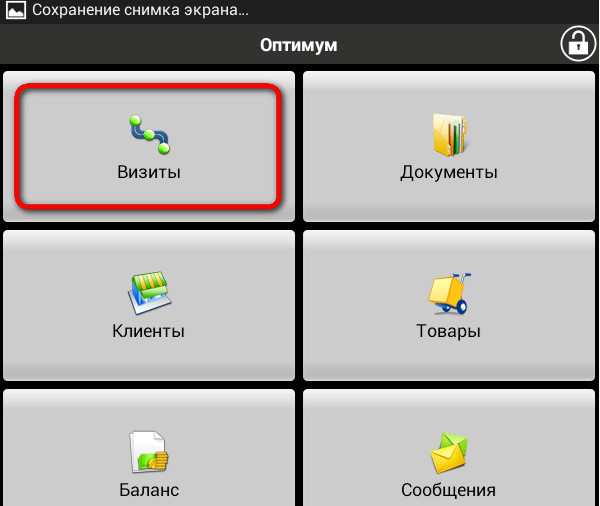
\includegraphics[width=0.8\linewidth]{scr10.jpg}}
		\ffigbox{\caption{Выбор торговой точки}\label{pic:pic11}}%
		{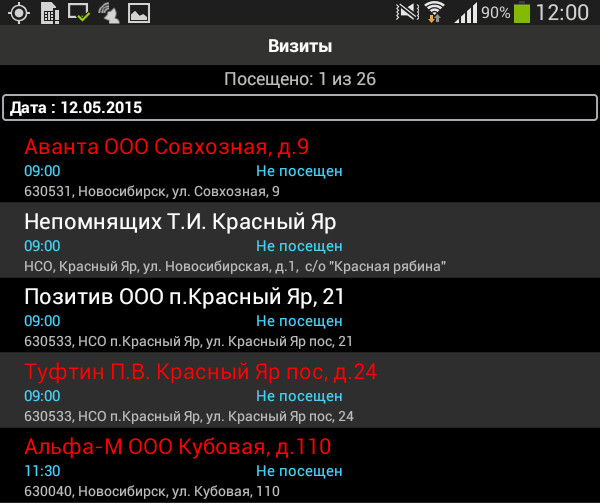
\includegraphics[width=0.8\linewidth]{scr11.jpg}}         
	\end{floatrow}
\end{figure}
\item Торговый представитель попадает в раздел «Визиты»
\footnote{Раздел «Визиты» предназначен для работы с маршрутами торгового представителя. "Визит" в системе "Оптимум" нужно рассматривать как факт посещения торговой точки за дату.} программы «Оптимум»
%То есть, несмотря на то, что фактически торговый представитель мог за день посетить данную ТТ несколько раз, в Системе будет зафиксирован один визит в данную ТТ (независимо от числа созданных документов и количества сеансов синхронизации с сервером).
(рис.\ref{pic:pic11}) и может выбрать необходимую торговую точку.
(подробно о визитах см.раздел\ref{sec:sec14_1})

Маршрут - это список посещений (визитов) клиентов торговым представителем на текущую дату. У мобильного сотрудника имеется возможность создать внеплановый визит в ТТ.
(см.\ref{sec:sec11_1})

\item Далее торговый представитель выбирает нужную ТТ, выполняет  «длительное нажатие»  (порядка 1-1,5 сек) и в открывшемся меню выбирает «Изменить статус»\label{it:it1}
(рис.\ref{pic:pic12})
\begin{figure}[!h]
\begin{floatrow}
	\ffigbox{\caption{Изменение статуса}\label{pic:pic12}}%
	{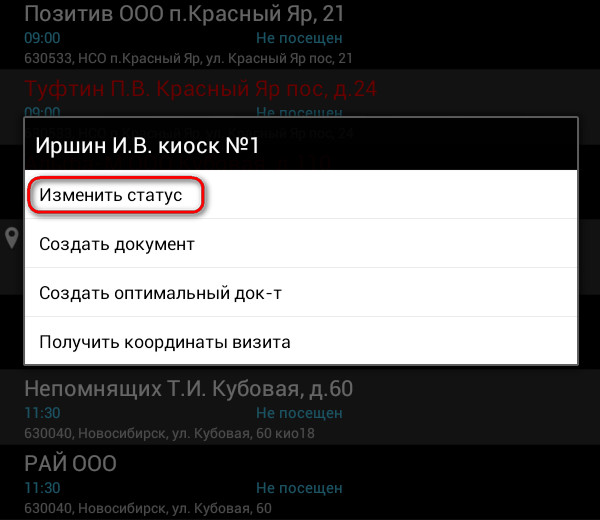
\includegraphics[width=0.8\linewidth]{scr12.jpg}}
	\ffigbox{\caption{Начало визита}\label{pic:pic13}}%
	{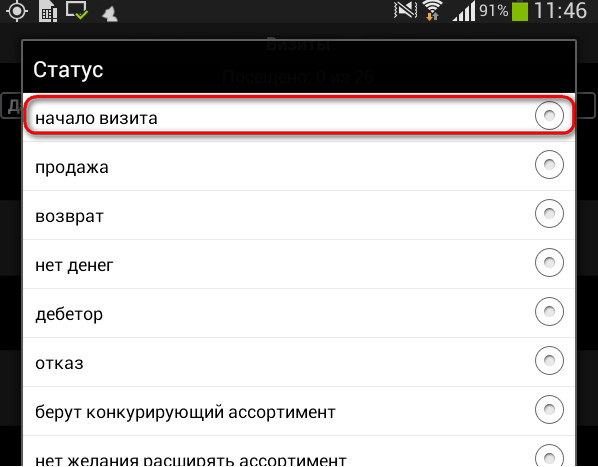
\includegraphics[width=0.8\linewidth]{scr13.jpg}}         
\end{floatrow}
\end{figure}
\item В следующем открывшемся меню выбирает «начало визита»\label{it:it2} 
(рис.\ref{pic:pic13})
\item Далее торговый представитель вновь выбирает нужную ТТ, выполняет  «длительное нажатие»  и в открывшемся меню выбирает «Получить координаты визита» . В случае если  и спутники обнаружены, текущие GPS-координаты торговой точки будут записаны в базу данных Мобильной части. Занимает данная процедура по времени не более 25 сек.\label{it:it3}
(рис.\ref{pic:pic14})
\begin{figure}[!h]
	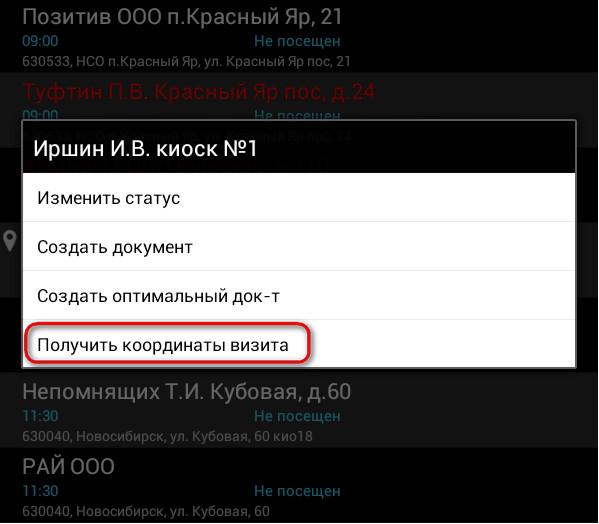
\includegraphics[width=0.4\linewidth]{scr14.jpg} 
	\caption{Получение координат визита}\label{pic:pic14}
\end{figure}

\item Когда координаты получены верно, на экране планшета рядом с наименованием ТТ в маршрутном листе слева сбоку должен появиться символ «капли»(1) ,его наличие говорит о том, что координаты визита получены и можно начинать работу. Так же изменился статус визита (2).
В противном случае если координаты визита получить не удалось, на экране будет появляться сообщение о том , что «координаты определить не удалось» в таком случае  повторяем пункт \ref{it:it2_1}
(рис.\ref{pic:pic15})
\begin{figure}[!h]
	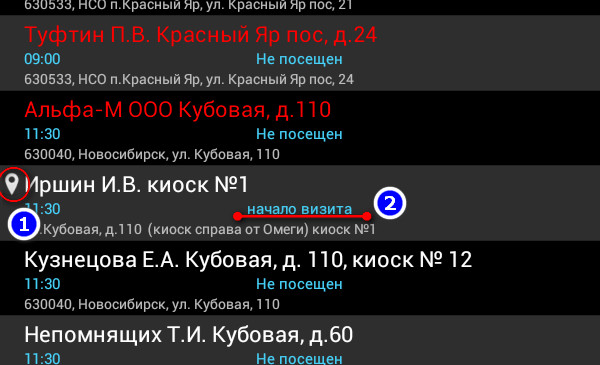
\includegraphics[width=0.5\linewidth]{scr15.jpg} 
	\caption{Координаты визита получены}\label{pic:pic15}
\end{figure}
\item Если GPS модуль включён, но координаты так и не определяются, необходимо определить координаты после окончания визита в ТТ, находясь на улице непосредственно на территории ТТ. воспользовавшись пунктом \ref{it:it2_1}

\item Затем торговый представитель заходит непосредственно в точку и выполняет там необходимые действия

\item \label{sec:sec3_1} Торговый представитель оформляет заказ. Для этого необходимо выполнить «длительное нажатие»  на ТТ с которой происходит работа  и из появившегося меню выбрать пункт «Создать документ»
(рис.\ref{pic:pic17})
\begin{itemize}
\item Выбрать тип создаваемого документа и произвести с ним необходимую работу.
(рис.\ref{pic:pic18})
\begin{figure}[!h]
	\begin{floatrow}
		\ffigbox{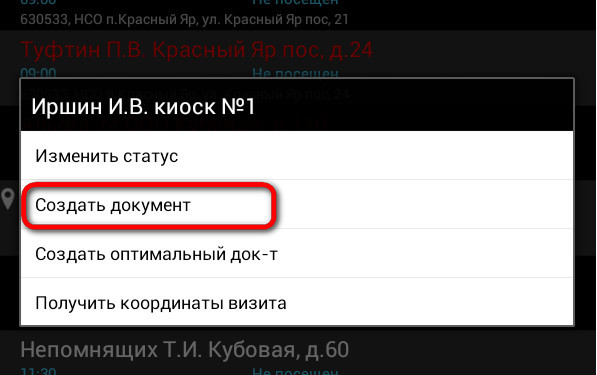
\includegraphics[width=0.9\linewidth]{scr17.jpg}}%
		{\caption{Создание документа}\label{pic:pic17}}
		\ffigbox{\caption{Выбор типа документа}\label{pic:pic18}}%
		{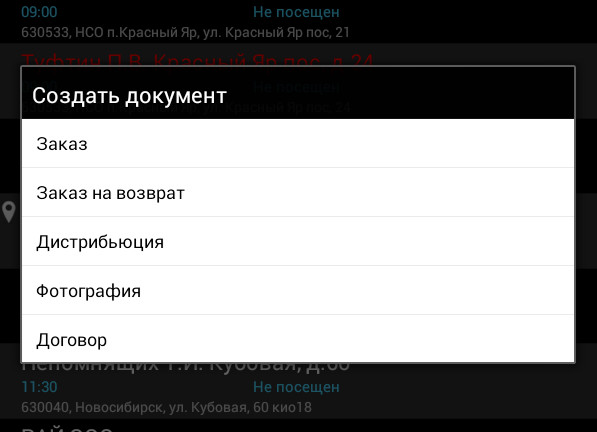
\includegraphics[width=0.8\linewidth]{scr18.jpg}}         
	\end{floatrow}
\end{figure}
\item Открывается окно просмотра заголовка документа.Вид и состав данных в окне заголовка документа зависит от типа документа, с которым идет работа в текущий момент. Помимо полей заголовка документа в этом окне так же отображаются атрибуты документа. 
В заголовке документа может быть не выбран <<тип оплаты>>.
(рис.\ref{pic:pic20})
\begin{figure}[!h]
	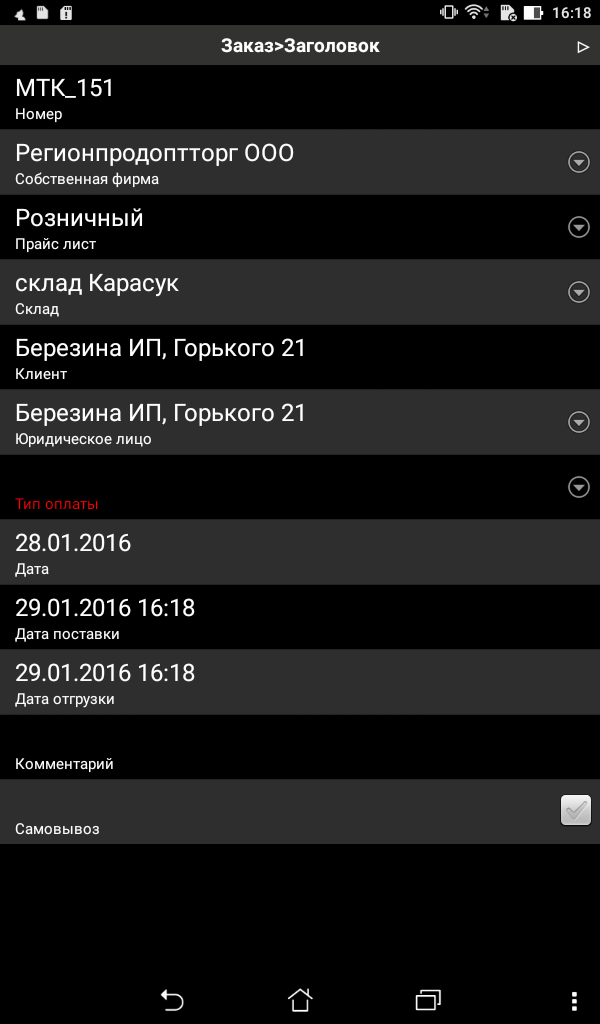
\includegraphics[width=0.25\linewidth]{scr20.png} 
	\caption{Шапка документа}\label{pic:pic20}
\end{figure}

\item Выбирается необходимый тип оплаты, если он не выбран.
(рис.\ref{pic:pic21})
\item Теперь шапка документа с заполненным типом оплаты. Необходимо нажать стрелку вправо (1), либо нужно совершить скользящее касание экрана слева – направо. 
Это позволит перейти к заполнению документа.
(рис.\ref{pic:pic22})
\begin{figure}[!h]
	\begin{floatrow}
		\ffigbox{\caption{Возможные типы оплаты}\label{pic:pic21}}%
		{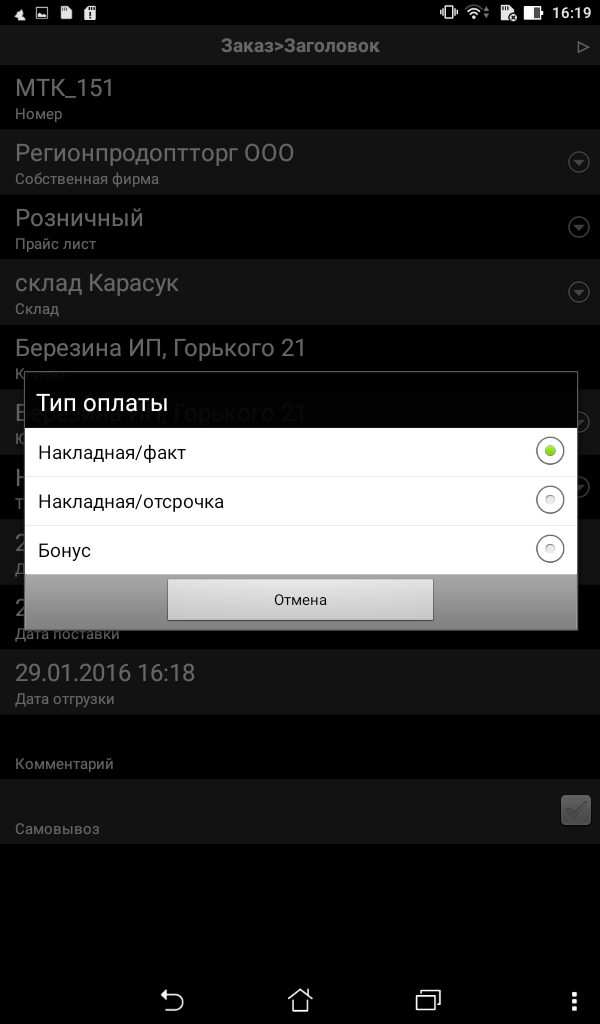
\includegraphics[width=0.6\linewidth]{scr21.png}}
		\ffigbox{\caption{Шапка документа с типом оплаты}\label{pic:pic22}}%
		{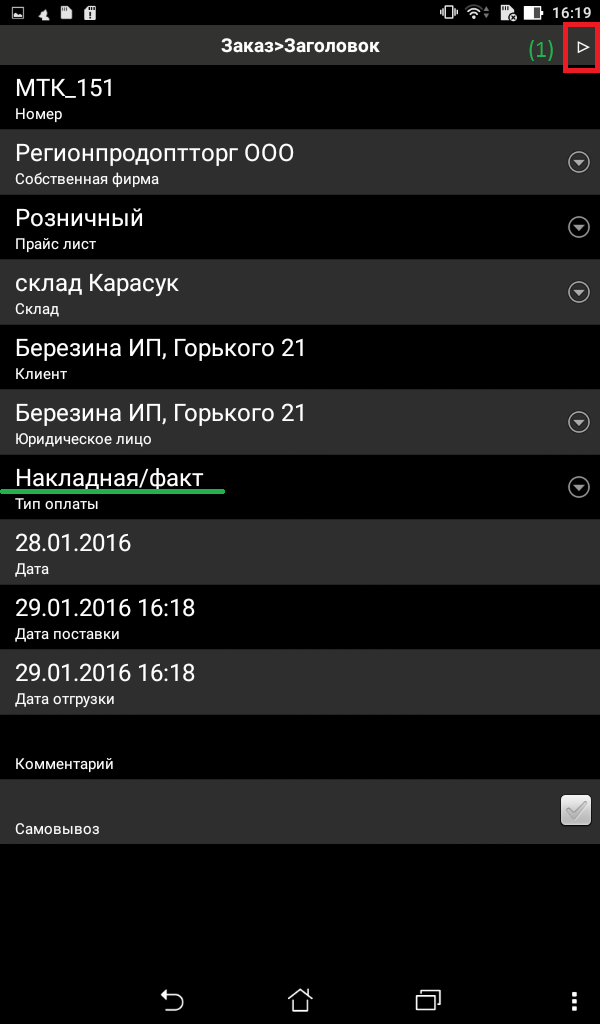
\includegraphics[width=0.6\linewidth]{scr22.png}}         
	\end{floatrow}
\end{figure}

\item Окрывается документ.
(рис.\ref{pic:pic23})
Экран с позициями может незначительно видоизменяться в зависимости от типа документа.В списке позиций присутствуют дополнительные справочные данные по позиции, такие как остаток на центральном складе и цена. 
При удержании элемента осуществляется переход к форме просмотра детальной информации о товарах. 
%\begin{figure}[h!]
%	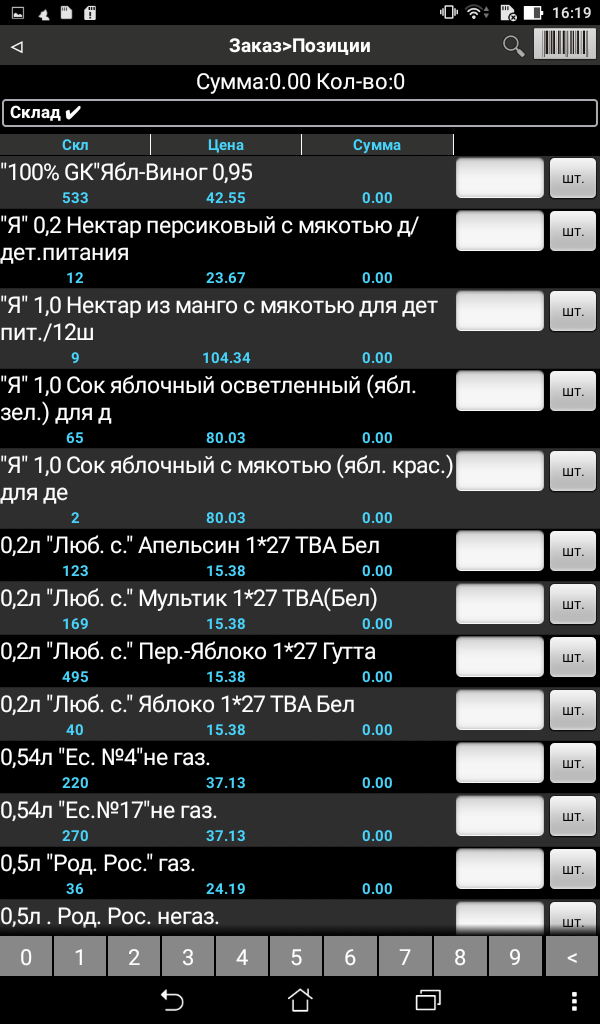
\includegraphics[width=0.3\linewidth]{scr23.png} 
%	\caption{Документ}\label{pic:pic23}
%\end{figure}
\item Далее в документе выбираются нужные позиции и проставляются количества товара.
(рис.\ref{pic:pic24})
\item Если всё сделано правильно, то при закрытии документа, на запрос, выбираем <<сохранить>>.
(рис.\ref{pic:pic25})
\begin{figure}[!h]
	\begin{floatrow}[3]
		\ffigbox{\caption{Документ}\label{pic:pic23}}%
		{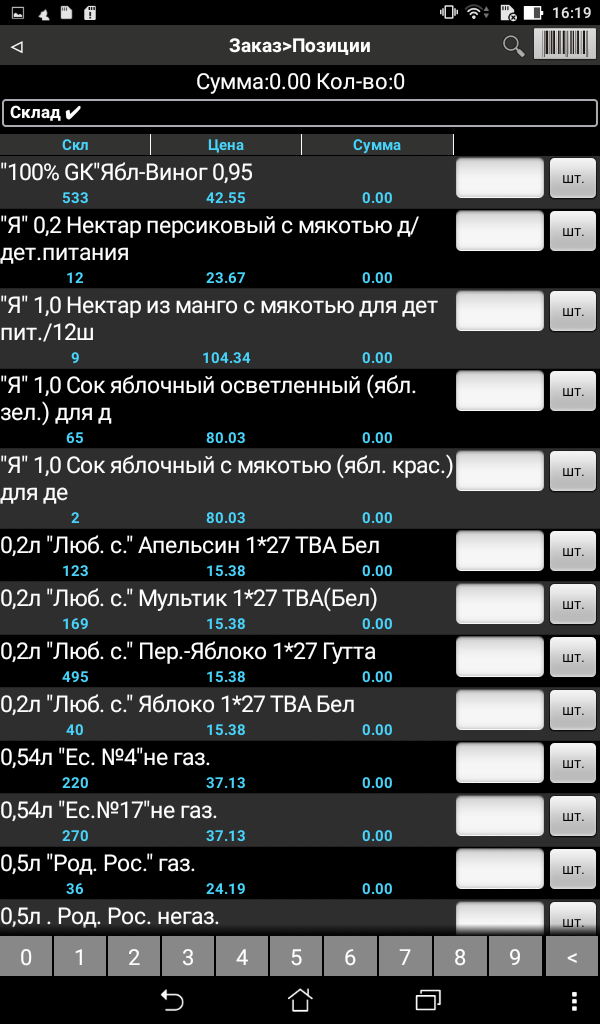
\includegraphics[width=0.8\linewidth]{scr23.png}}
		\ffigbox{\caption{Заполнение документа}\label{pic:pic24}}%
		{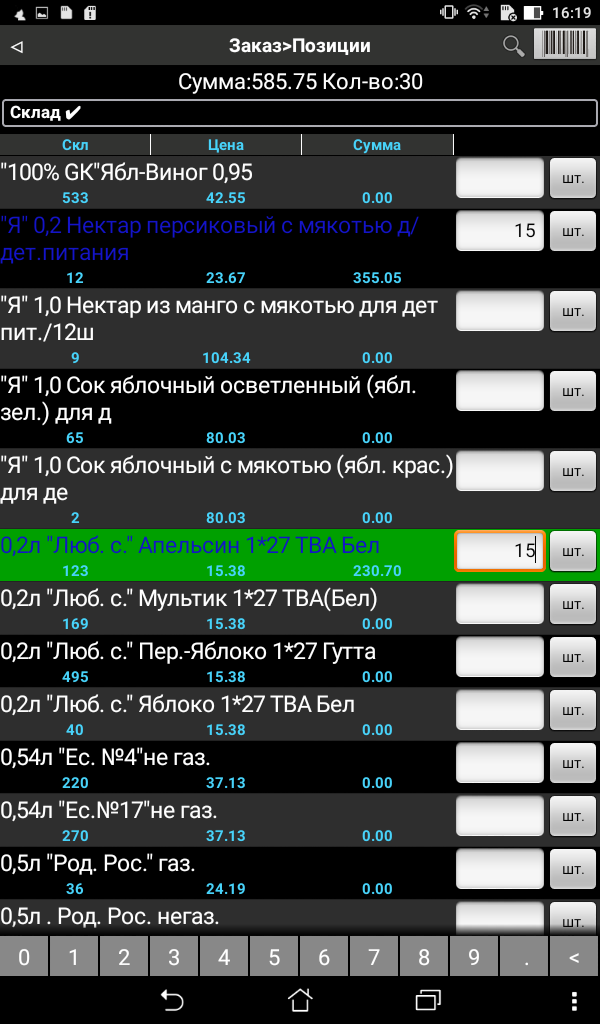
\includegraphics[width=0.8\linewidth]{scr24.png}}
		\ffigbox{\caption{Закрытие документа}\label{pic:pic25}}%
		{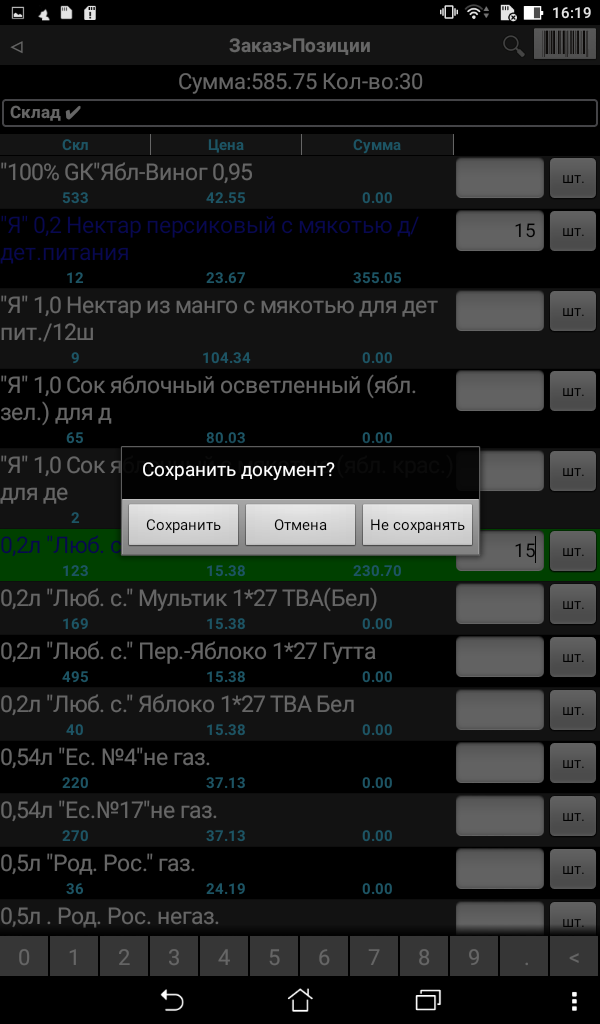
\includegraphics[width=0.8\linewidth]{scr25.png}}         
	\end{floatrow}
\end{figure}

\item Теперь созданный документ появится в списке документов.
(рис.\ref{pic:pic26})
\item Торговый представитель создаёт документ (рис.\ref{pic:pic18}) «Фотография»
и выполняет фотографирование  ассортимента представленного в ТТ.
(рис.\ref{pic:pic19})
\begin{figure}[!h]
	\begin{floatrow}
		\ffigbox{\caption{Список документов}\label{pic:pic26}}%
		{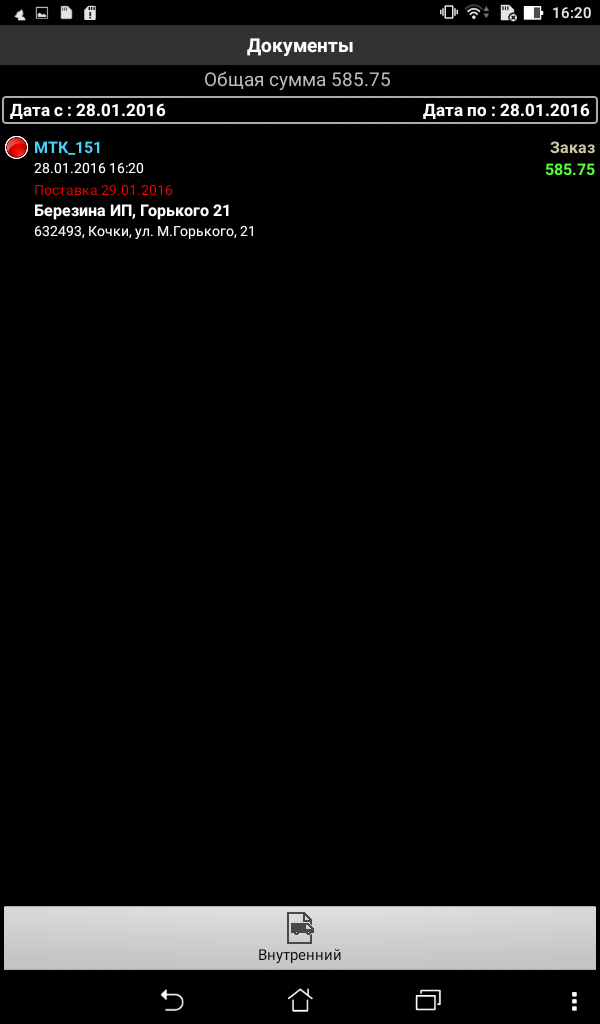
\includegraphics[width=0.6\linewidth]{scr26.png}}
		\ffigbox{\caption{Выбор типа для фотографии}\label{pic:pic19}}%
		{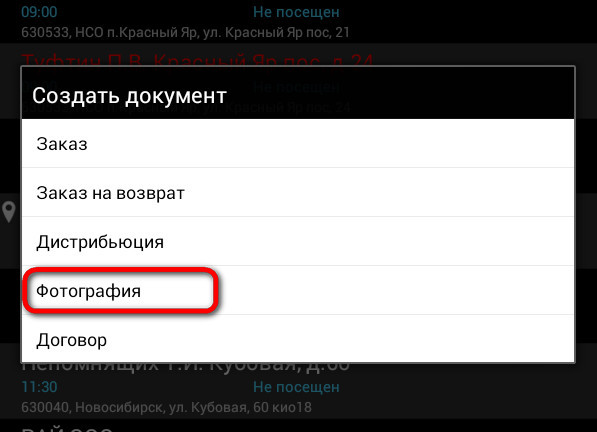
\includegraphics[width=0.8\linewidth]{scr19.jpg}}         
	\end{floatrow}
\end{figure}
\item Открывается документ «Фотография».Необходимо нажать стрелку вправо (1). Это позволит перейти к заполнению документа.
(рис.\ref{pic:pic27})
\item В открывшемся документе нажимаем кнопку <<добавить>>.
(рис.\ref{pic:pic29})
\begin{figure}[!h]
	\begin{floatrow}
		\ffigbox{\caption{Список документов}\label{pic:pic27}}%
		{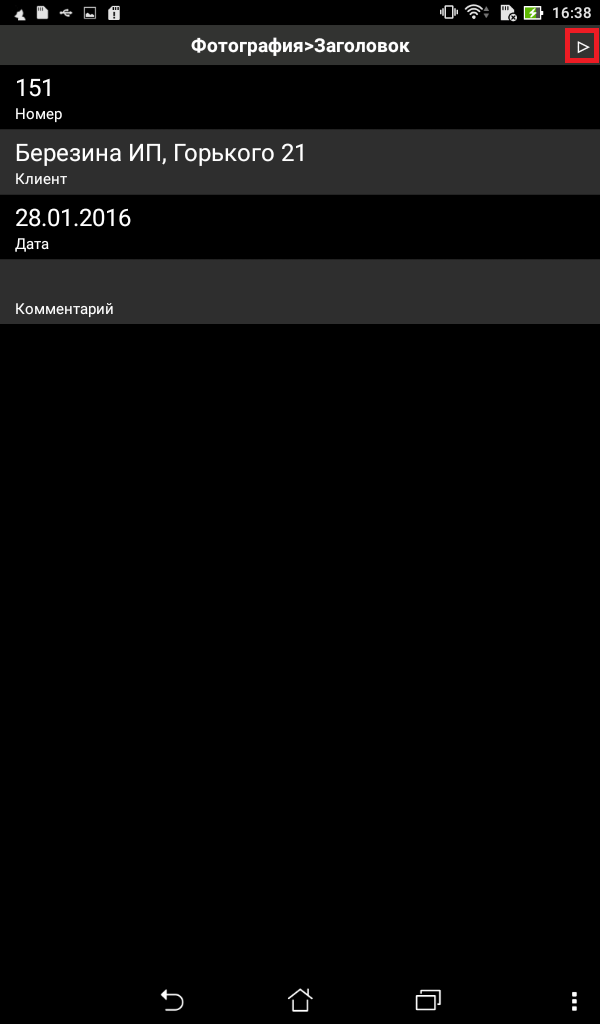
\includegraphics[width=0.6\linewidth]{scr27.png}}
		\ffigbox{\caption{Кнопка добавить фотографию}\label{pic:pic29}}%
		{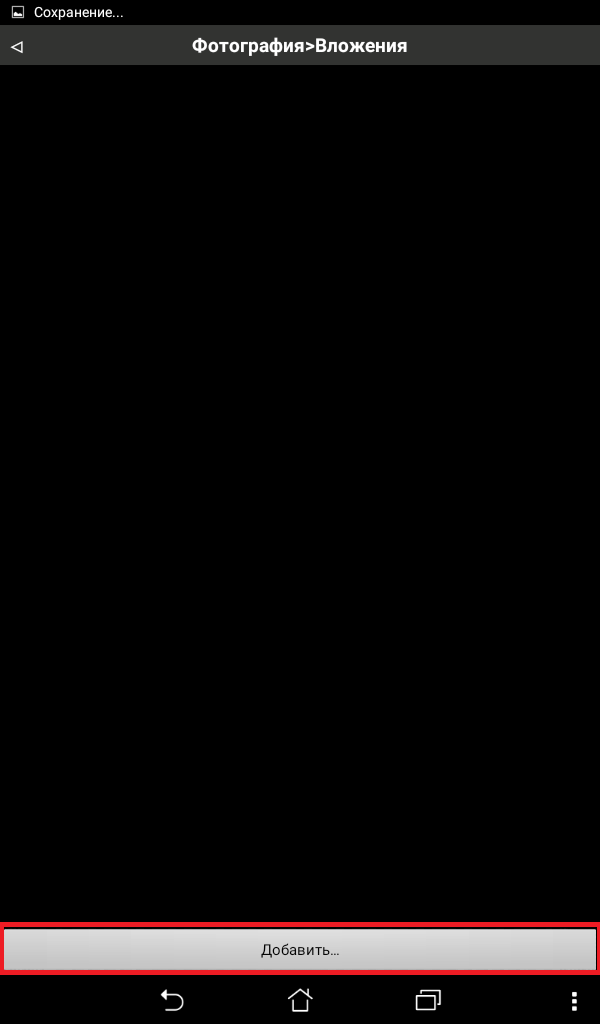
\includegraphics[width=0.6\linewidth]{scr29.png}}         
	\end{floatrow}
\end{figure}



\item КПК переходит в режим фотографирования. Выбираем необходимый план и фотографируем.
(рис.\ref{pic:pic30})
\begin{figure}[!h]
	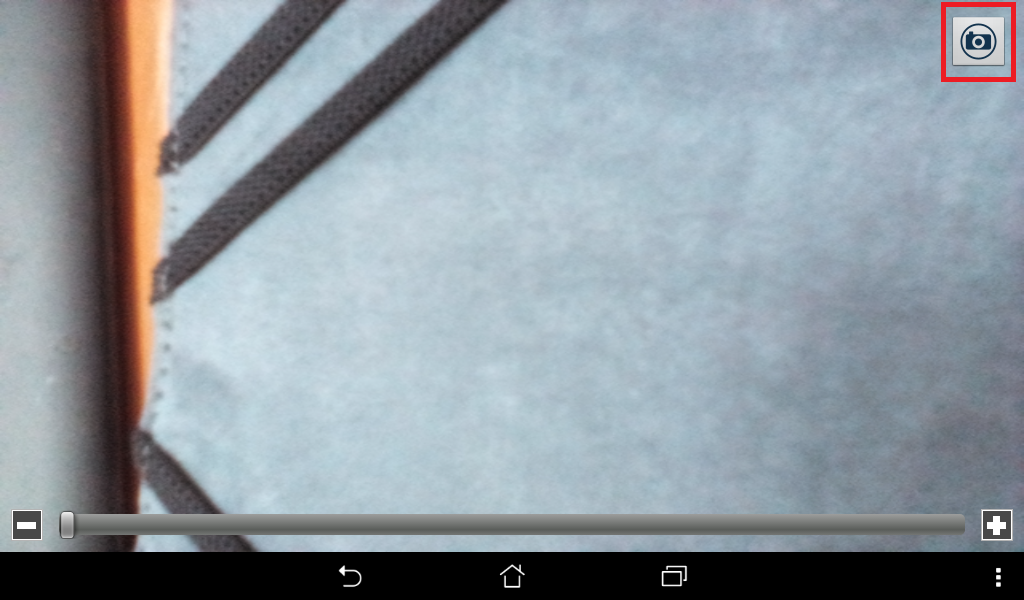
\includegraphics[width=0.5\linewidth]{scr30.png} 
	\caption{Фотография}\label{pic:pic30}
\end{figure}
\item Для прикрепления ещё одной фотографии выполните описанные действия снова (кнопка «Добавить…»)
\item Для удаления фотографии нажмите на файле соответствующей фотографии и в открывшемся окне нажмите на кнопку «Удалить».
\item Размер фотографий задаётся в модуле Настройки. 
  

\end{itemize}

\item По окончанию визита необходимо запустить процесс синхронизации описанный в п.\ref{it:it2_1} по \ref{it:it2_2}

\item В случае, если при посещении ТТ торговым представителем не был оформлен заказ для этой ТТ, агенту необходимо, находясь ещё на территории данной ТТ поменять статус посещения (п.\ref{it:it1}) ТТ на необходимый: «Дебитор», «Нет денег», «Товар в наличии» или иные причины.
\item Переход к определённой позиции документа\\
При формировании документа в момент ввода количественных данных по товарным позициям у сотрудника может возникнуть потребность в быстром переходе к той или иной товарной позиции в большом списке товаров. Для этого предусмотрена специальная функция, которую можно вызвать из общего меню, нажав на кнопку \textbf{Перейти к....} 

\includegraphics[width=0.03\linewidth]{scr_cm.png} 
После запуска функции перехода откроется окно выбора вариантов поиска: поиск по краткому наименованию объекта, по полному наименованию или по внешнему коду объекта. Выбрав наиболее подходящий вариант, необходимо в нижней части окна ввести символы, по которым будет вестись поиск конкретной товарной позиции.
\item Акцептование/разакцептование документа\\
В рамках Системы термин \textbf{Акцептование} означает перевод документа в состояние, в котором его редактирование или удаление недоступно пользователю. 
\item Удаление документа\\
В мобильной части Системы предусмотрено удаление акцептованных и неакцептованных документов, которые не были переданы в серверную часть. Неакцептованные документы всегда доступны для удаления.Документы, переданные в серверную часть недоступны для удаления в любом случае.
Для того чтобы удалить документ, выполните следующие действия:
\begin{itemize}
	\item В модуле \textbf{Документы} выберите документ и откройте его контекстное меню;
	\item В контекстном меню выберите пункт \textbf{Удалить документ};
\end{itemize}
Выбранный документ будет удален.
\end{enumerate}